%----------------------------------------------------------------------------------------
%	PROGETTAZIONE
%----------------------------------------------------------------------------------------

\section{Progettazione}
Una volta chiarificati tutti i requisiti ed i desiderata del cliente, si è passati alla fase di progettazione. Inizialmente si è preferito astrarre dalle tematiche di "basso livello" dando priorità alla definizione di tutti i servizi necessari per il corretto funzionamento del sistema. Nello specifico si parla di microservizi, infatti ogni componente software da sviluppare modella un insieme specifico di concetti, precedentemente identificati nei 9 sottodomini. Un aspetto di cruciale importanza è definire a monte le modalità di interazione tra i vari servizi. Per ognuna di queste è necessario specificare il "fornitore" (\textit{upstream}) ed il "consumatore" (\textit{downstream}), così da stabilire una dipendenza tra le coppie di servizi che vincoli una delle parti ad adattarsi alle regole operative dell'altra.

\begin{figure}[H]
    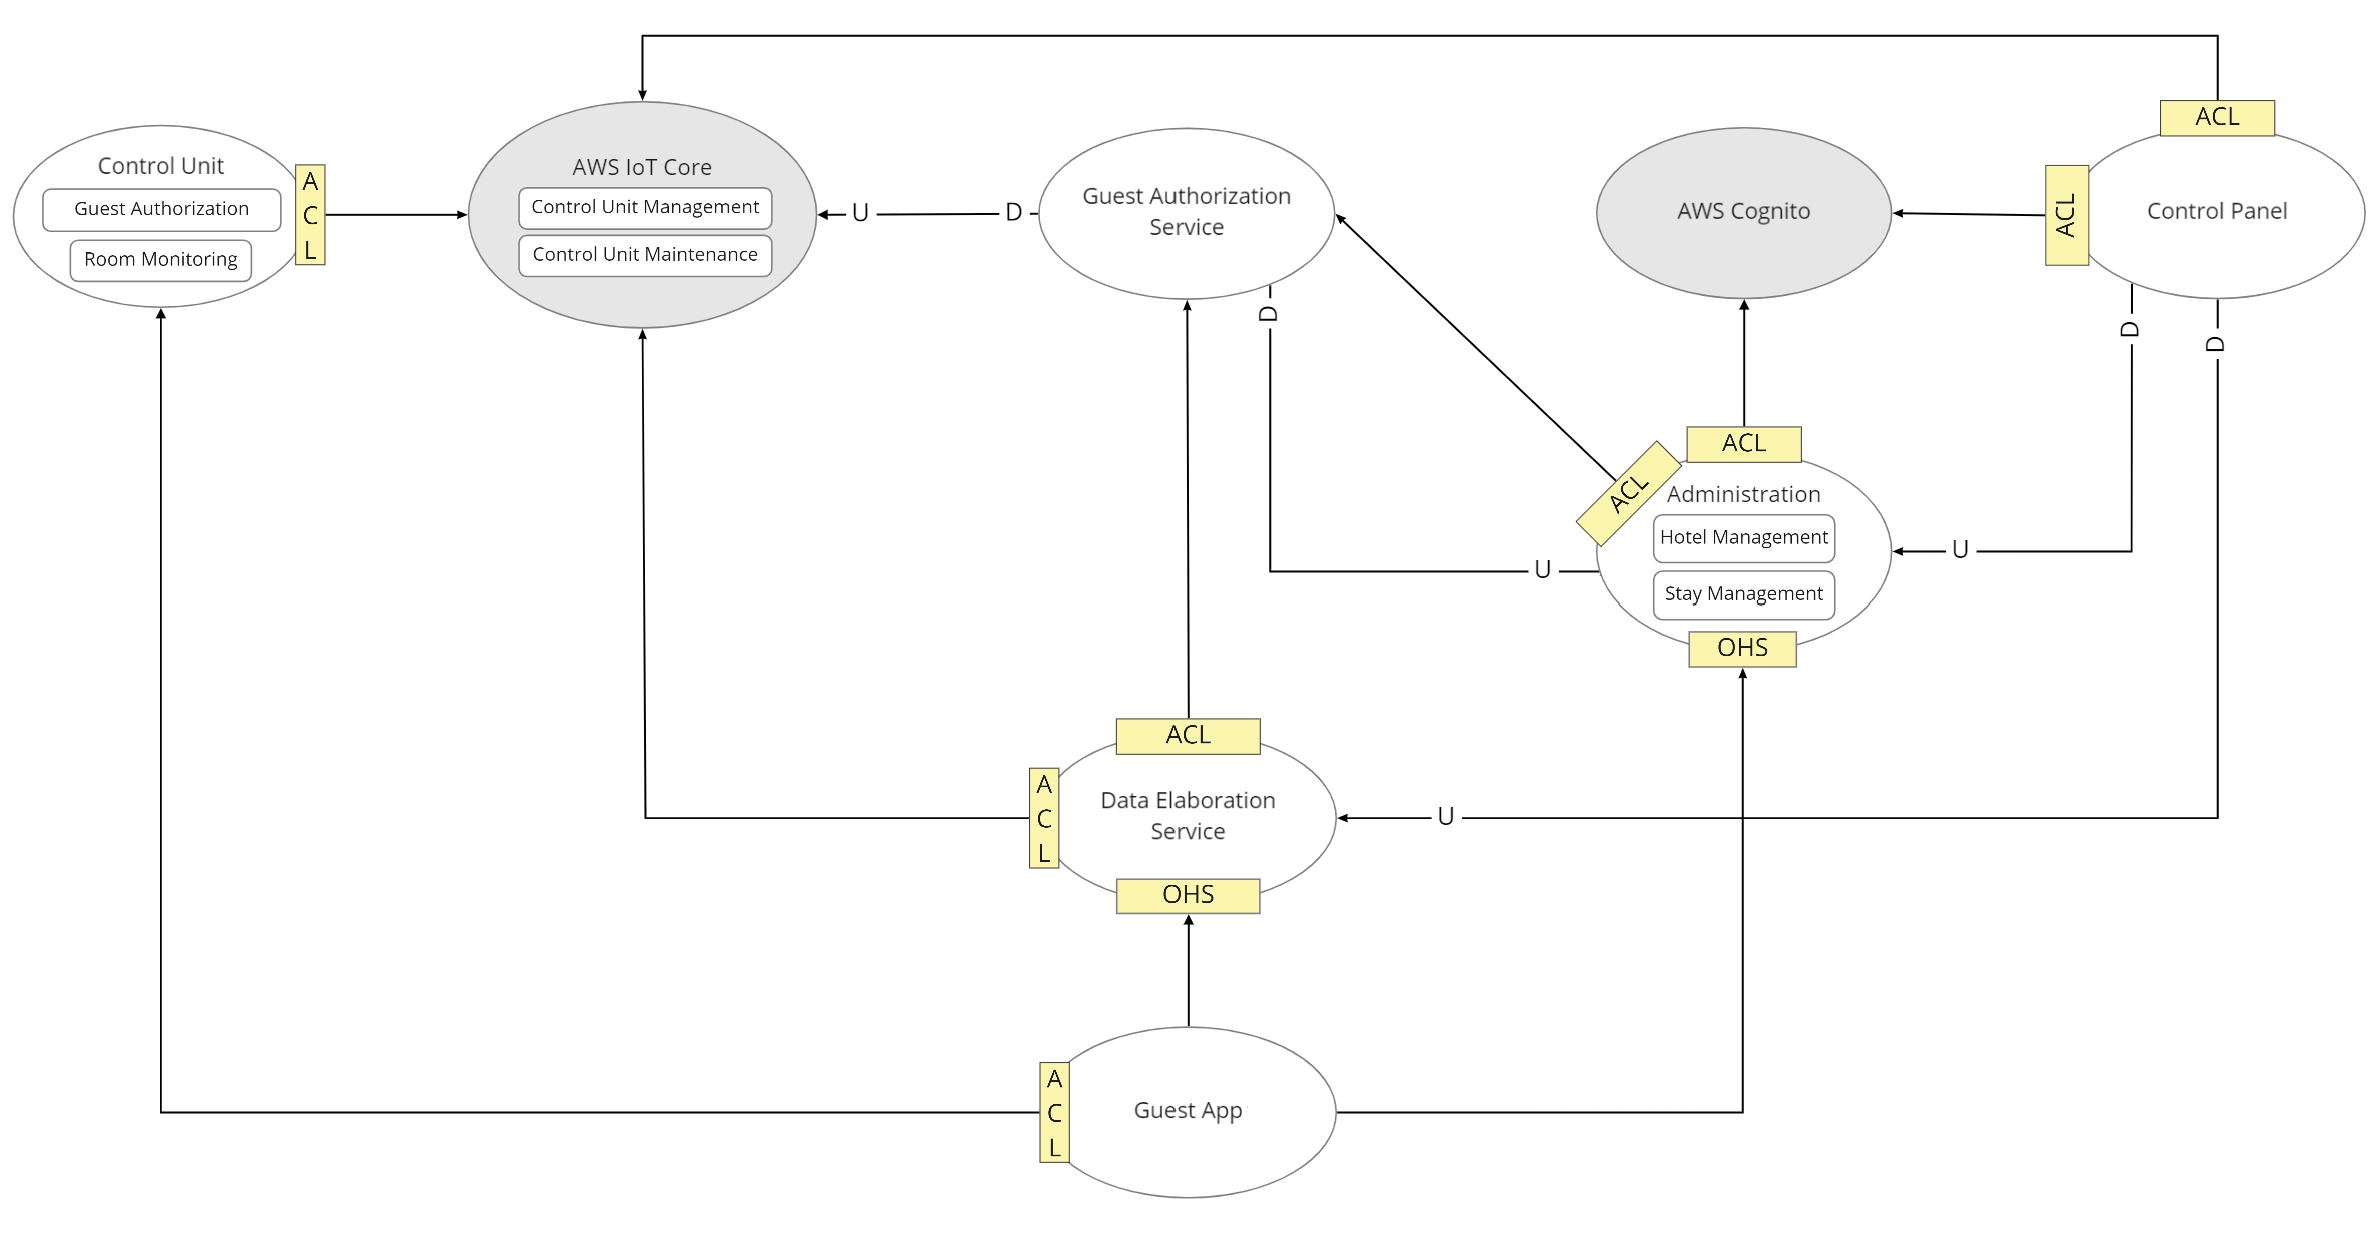
\includegraphics[width=\textwidth]{context-map.png}
    \centering
    \caption[contextmap]{Schema dei microservizi che compongono Ecotrip}
    \label{fig:contextmap}
\end{figure}

Le componenti del sistema Ecotrip (Figura \ref{fig:contextmap}) possono essere schematizzate in:
\begin{itemize}
    \item \textbf{Administration}: servizio che modella  i concetti e implementa le funzionalità di gestione degli hotel (\textit{Hotel Management}) e dei pernottamenti (\textit{Stay Management}).  Entrambe queste API necessitano di verificare l'autenticità delle richieste, per questo Administration dipende sia da AWS Cognito e che da Guest Authorization Service, il quale genera i \textit{token} usati da Guest App per eseguire le richieste. Queste due dipendenze in realtà non rappresentano connessioni con i servizi remoti in quanto le verifiche possono essere eseguite localmente ad Administration, tuttavia il processo di validazione è vincolato alle tecnologie usate dai rispettivi servizi. La comunicazione verso i servizi di AWS Cognito e Guest Authorization sarà regolamentata da opportuni \textit{adapter} (ACL) che consentono di convertire, sia in entrata che in uscita, i concetti di dominio esterni in quelli interni al servizio stesso.  
    Poiché è richiesto che il pannello di controllo sia fruibile via web, si applica il \textit{backend-for-frontend pattern}: Administration si occuperà di fornire una RESTful API ad uso del \textit{frontend} che sarà descritto in seguito.
    Si è quindi evitata una logica a microservizi pura in quanto:
    \begin{itemize}
        \item il ciclo di vita può essere unito in modo da avere un unico deployment su unica infrastruttura riducendo i costi di fornitura del servizio;
        \item Hotel Management avrà un numero di richieste sempre molto basso e lo \textit{scaling} del servizio può essere dimensionato pensando solamente a Stay Management.
    \end{itemize}
    L'alternativa a questa strategia è di separare i due servizi e progettarli con paradigma totalmente \textit{serverless}, che renda i costi del servizio proporzionali all'utilizzo. Questa modalità però dipende strettamente dai servizi offerti dal \textit{cloud provider} e richiederebbe uno studio più approfondito dello stesso, cosa che non è possibile affrontare in questa sede.
    \item \textbf{AWS Cognito}: rappresenta il sottodominio relativo all'autenticazione, cioè tutte le funzionalità che consento di gestire gli \textit{account} degli amministratori di sistema e degli \textit{hotelier}, che può essere demandato in \textit{out-sourcing}. Una possibile soluzione può essere Amazon AWS Cognito.
    \item \textbf{Control Panel}: realizza la logica di business \textit{frontend} dei sottodomini Administration e Authentication, nella pratica si andrà a realizzare una \textit{web app} sfruttando il framework React.js. Questa delegherà l'autenticazione e la gestione degli account creati ad AWS Cognito. Inoltre, il pannello di controllo risultante dovrà permettere di visualizzare sia lo stato dalle centraline che i dati prodotti da queste. Ciò comporta la creazione di un collegamento tra il Control Panel ed i servizi AWS IoT Core e Data Elaboration Service.
    \item \textbf{AWS IoT Core}: include i sottodomini Control Unit Management, Control Unit Maintenance e lo \textit{storage cloud} dei dati generati da Room Monitoring. Come per l'autenticazione, la sua implementazione può essere delegata a un fornitore esterno, nel caso specifico si è scelto l'omonimo servizio di amazon AWS IoT Core. Quest'ultimo dispone di un pannello di controllo con cui poter agevolmente eseguire tutti i \textit{task} richiesti, per esempio permette di abbinare le centraline alle stanze attraverso \textit{tagging}. Infine, tramite un'apposita Rest API, per ogni centralina si è in grado di ottenere i dati caricati, verificarne lo stato ed inviare dei comandi da remoto: funzionalità che può essere sfruttata per inviare il token di un ospite.
    \item \textbf{Guest Authorization}: realizza funzionalità che possono essere circoscritte in due sistemi distinti. Il primo è Guest Authorization Service, il quale si occupa della generazione del \textit{token}, a seguito della creazione di un nuovo soggiorno (eventi di \textit{check in} e \textit{check out}) da parte del servizio di Stay Management, e del suo invio verso la centralina tramite AWS IoT Core. Il secondo sistema verrà incluso come modulo all'interno del software della centralina.
    \item \textbf{Control Unit}: rappresenta il software installato sulla centralina, il quale si compone di due moduli, il primo (Room Monitoring) si occupa del monitoraggio dei consumi, mentre il secondo (Guest Authorization) è dedicato alla gestione del \textit{transponder NFC}. La Control Unit oltre a ricevere gli aggiornamenti di stato da AWS IoT Core, vi inoltra i dati raccolti dai sensori. Come fatto per Administration, anche in questo caso si è evitato di creare due software indipendenti al fine di avere lo stesso ciclo di vita e un unico \textit{deployment} che possa semplificare le attività di configurazione e manutenzione della centralina.
    \item \textbf{Guest App}: realizza un applicativo lato \textit{frontend} che comunica con la Control Unit per ottenere il \textit{token} da presentare al servizio di Data Elaboration per accedere ai dati del pernottamento.
\end{itemize}

Di seguito viene proposto un approfondimento su ogni componente appena elencata.

\subsection{Control Unit}
Nel caso specifico della centralina la fase di progettazione coinvolge sia la componente \textit{hardware} che quella \textit{software}. L'elemento \textit{core} del prototipo è una scheda \textit{raspberry pi 4B} alla quale sono connessi i sensori precedentemente citati nella sezione dei requisiti. Data la finalità prototipale e le tempistiche ristrette si predilige l'acquisto di un set di sensori che siano disponibili nell'immediato, preferibilmente digitali e con un supporto software adeguato. Ovviamente, di questi si verificherà anche l'accuratezza nonostante non sia ritenuto un aspetto fondamentale durante questa fase di progetto. 

\subsubsection{Hardware}
Dopo un'attenta fase di ricerca e un confronto tra le diverse soluzioni, si opta per l'acquisto di un determinato set di sensori, presentato e approfondito nella sezione corrente. Di ciascuno verrà fornita una breve descrizione che include le caratteristiche tecniche principali, mentre i dettagli relativi alla componente software saranno trattati nella sezione successiva.\newline\newline
%
\textbf{ICQUANZX PN532 NFC}\footnote{Link al venditore: \href{https://www.amazon.it/ICQUANZX-Communication-Arduino-Raspberry-Android/dp/B07VT431QZ/}{https://www.amazon.it/ICQUANZX}}: modulo di trasmissione altamente integrato per la comunicazione NFC (Near Field Communication) a 13.56 MHz. Il sensore è dotato di un interruttore con il quale è possibile cambiare la modalità scegliendo tra I2C, SPI e UART. Inoltre, il modulo supporta la lettura/scrittura RFID e possiede 4 fori di montaggio da 3mm. 
    
    \begin{table}[H]
        \centering
        \begin{tabular}{|l|l|}
        \hline
        \textbf{Caratteristica}     & \textbf{Descrizione}                      \\ \hline        Protocollo di comunicazione                   & I2C\footnote{Per dettagli: \url{https://www.i2c-bus.org/}}, SPI and HSU (High Speed UART)                                                                                                                     \\ \hline
        Supporto RFID                                 & \begin{tabular}[c]{@{}l@{}}modalità in lettura o scrittura:\\   - Mifare 1k, 4k, Ultralight, and DesFire cards\\   - ISO/IEC 14443-4 card\end{tabular} \\ \hline
        Distanza di comunicazione                     & 5cm$\sim$7cm (PCB Antenna)                                                                                                                             \\ \hline
        Virtualizzazione                              & può funzionare come una carta virtuale                                                                                                                 \\ \hline
        Dimensioni                                    & 43mm x 41mm x 4mm                                                                                                                                          \\ \hline
        \end{tabular}
        \caption{\label{pn532-features}Caratteristiche principali del modulo PN-532.}

    \end{table}

    La modalità di funzionamento determina anche la configurazione a livello di circuito (alimentazione).
    \begin{table}[H]
        \centering
        \begin{tabular}{|c|c|}
        \hline
        \textbf{Interfaccia} & \textbf{Valore}                            \\ \hline
        VCC                & 3.3V$\sim$5V                              \\ \hline
        I2C/UART           & 3.3V$\sim$24V TTL                         \\ \hline
        SPI                & 3.3V TTL con 100 ohm di resistenza \\ \hline
        \end{tabular}
        \caption{\label{pn532-modalities}Modalità di funzionamento del modulo PN-532.}
    \end{table}
    
    \begin{figure}[H]
        \begin{center}
          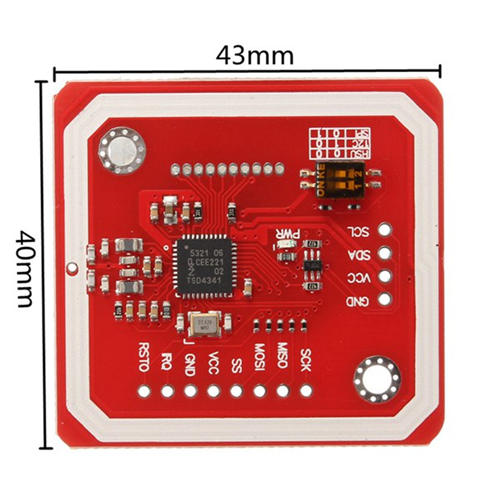
\includegraphics[width=0.35\textwidth]{images/sensors/pn532.png}
        \end{center}
        \caption{\label{pn532}Modulo PN532}
    \end{figure}
    
    
\textbf{GY-302 BH1750}\footnote{Link al venditore: \href{https://www.amazon.it/AZDelivery-Sensore-Intensità-Luminosità-Raspberry/dp/B07NLL4SCB}{https://www.amazon.it/AZDelivery-BH170}}: sensore digitale per il rilevamento della luminosità ambientale basato sull'interfaccia bus I2C; internamente monta un ADC. 

\begin{table}[H]
    \centering
    \begin{tabular}{|l|l|}
    \hline
    \textbf{Caratteristica}     & \textbf{Descrizione}                      \\ \hline    Alimentazione               & 3$\sim$5V                                 \\ \hline
    Protocollo di comunicazione & I2C                                       \\ \hline
    Output                      & segnale in uscita digitale (ADC build-in) \\ \hline
    Accuratezza                 & precisione elevata, vicino a 1 Lu         \\ \hline
    Data range                  & 0$\sim$65535                              \\ \hline
    Dimensioni                  & 13.9 x 18.5 mm                           \\ \hline
    \end{tabular}
    \caption{\label{bh1750-features}Caratteristiche principali del modulo BH1750.}
\end{table}
%
\begin{figure}[H]
    \begin{center}
      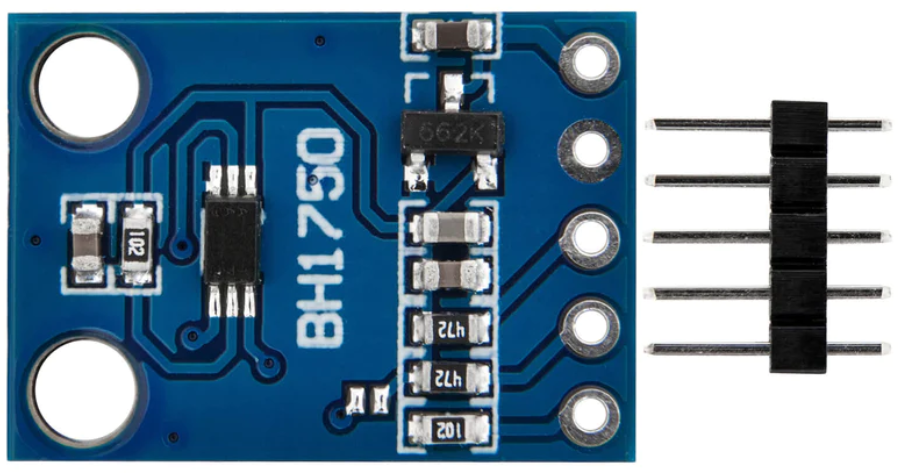
\includegraphics[width=0.35\textwidth]{images/sensors/bh1750.png}
    \end{center}
    \caption{Modulo BH1750}
\end{figure}
%
\textbf{ACS712 - 20A}\footnote{Link al venditore: \href{https://www.amazon.it/AZDelivery-corrente-sensore-Current-Raspberry/dp/B0736DYV3W?th=1}{https://www.amazon.it/AZDelivery-ACS712}}: sensore di corrente usato per misurare una corrente AC o DC in un range di ±5A con un errore di 1.5\% a T = 25 °C. Il sensore è composto da due parti, un collegamento per il chip del sensore, e l'altra parte con due connettori a morsettiera per la misurazione della corrente.
Il sensore utilizza l'effetto Hall per rilevare la corrente che lo attraversa. La corrente che fluisce attraverso il sensore genera un campo magnetico che viene rilevato dal sensore e convertito in una tensione analogica proporzionale.

\begin{table}[H]
    \centering
    \begin{tabular}{|l|l|}
    \hline
    \textbf{Caratteristica} & \textbf{Descrizione}                                \\ \hline
    Alimentazione           & 5V                                                  \\ \hline
    Tensione in uscita      & metà di quella di allimentazione (2.5V se Vcc = 5V) \\ \hline
    Output                  & segnale in uscita digitale (ADC build-in)           \\ \hline
    Dimensioni              & 89.9 x 59.9 x 20.1 mm                               \\ \hline
    \end{tabular}
    \caption{\label{acs712-features}Caratteristiche principali del modulo ACS712.}
\end{table}

\begin{figure}[H]
    \begin{center}
      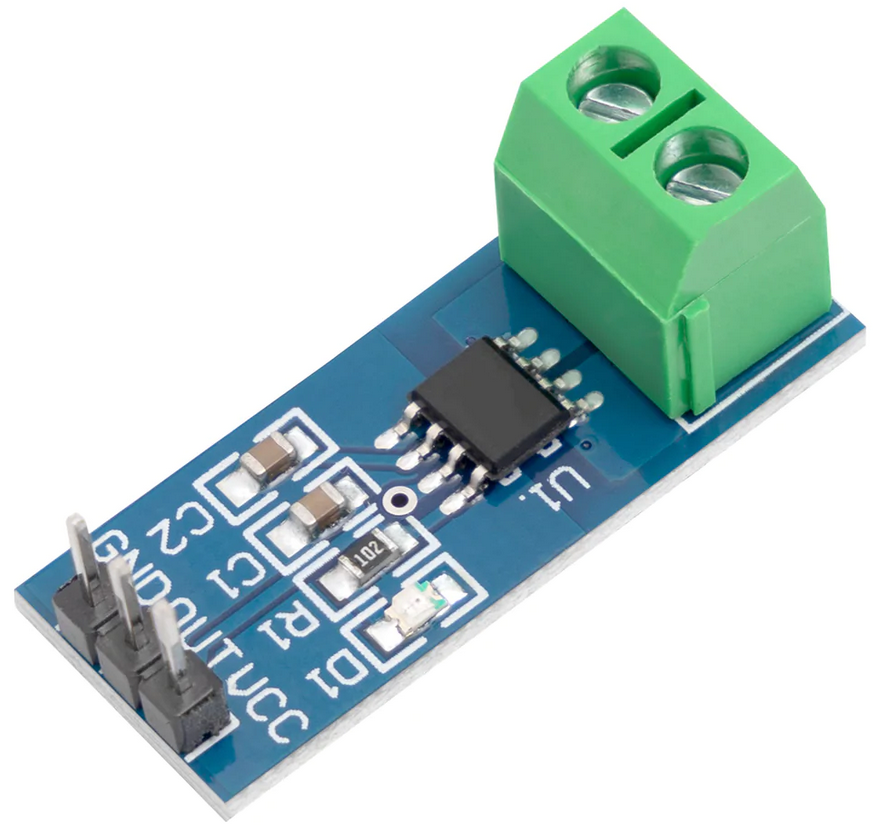
\includegraphics[width=0.35\textwidth]{images/sensors/acs712.png}
    \end{center}
    \caption{Modulo ACS712}
\end{figure}

\textbf{DHT22}\footnote{Link al venditore: \href{https://www.amazon.it/AZDelivery-temperatura-circuito-Raspberry-gratuito/dp/B078SVZB1X/ref=sr_1_6?keywords=dht22&qid=1673890614&sr=8-6&th=1}{https://www.amazon.it/AZDelivery-DHT22}}: sensore di umidità/temperatura relativa che emette un segnale digitale. Utilizza un sensore di umidità capacitivo e un termistore per misurare l'aria circostante. 

\begin{table}[H]
    \centering
    \begin{tabular}{|l|l|}
    \hline
    \textbf{Caratteristica} & \textbf{Descrizione}               \\ \hline
    Alimentazione           & 3$\sim$5V                          \\ \hline
    Tensione operativa max  & 2.5mA max                          \\ \hline
    Range umidità           & 0\% - 100\%  (accuratezza 2 - 5\%) \\ \hline
    Range di temperatura    & -40°C - 125°C (accuratezza ±0.5°C) \\ \hline
    Freq. di campionamento  & 0.5Hz (lettura ogni 2s)            \\ \hline
    Dimensioni              & 15 x 38 x 9 mm                     \\ \hline
    \end{tabular}
    \caption{\label{DHT22-features}Caratteristiche principali del modulo DHT22.}
\end{table}

\begin{figure}[H]
    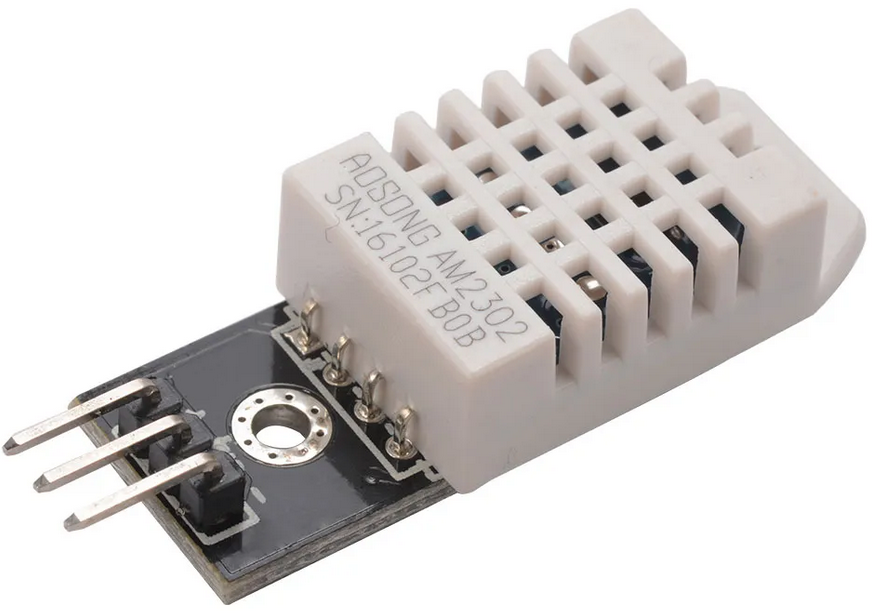
\includegraphics[width=.35\textwidth]{images/sensors/dht22-a.png}\hfill
    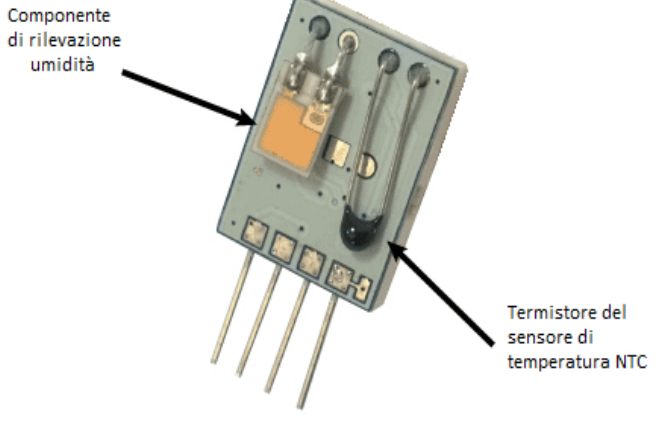
\includegraphics[width=.35\textwidth]{images/sensors/dht22-b.png}\hfill
    \caption{Modulo DHT22.}
\end{figure}


\textbf{ADS1115}\footnote{Link al venditore: \href{shorturl.at/btJVZ}{https://www.amazon.it/AZDelivery-ADS1115}}: convertitore da analogico a digitale, facilmente utilizzabile con una scheda Raspberry Pi utilizzando un bus di comunicazione I2C. Il convertitore ha una buona precisione poiché lavora a 16 bit e sfrutta 4 canali.  

\begin{table}[H]
    \centering
    \begin{tabular}{|l|l|}
    \hline
    \textbf{Caratteristica}   & \textbf{Descrizione} \\ \hline
    Alimentazione             & 2.0$\sim$5.5V        \\ \hline
    Tipo di interfaccia       & I2C                  \\ \hline
    Bit rate ADC              & 16 bit               \\ \hline
    Canali                    & AN0, AN1, AN2, AN3   \\ \hline
    Amplificatore di guadagno & programmabile        \\ \hline
    Dimensioni                & 90 x 52 x 10 mm      \\ \hline
    \end{tabular}
    \caption{\label{ADS1115-features}Caratteristiche principali del modulo ADS1115.}
\end{table}

\begin{figure}[H]
    \centering
    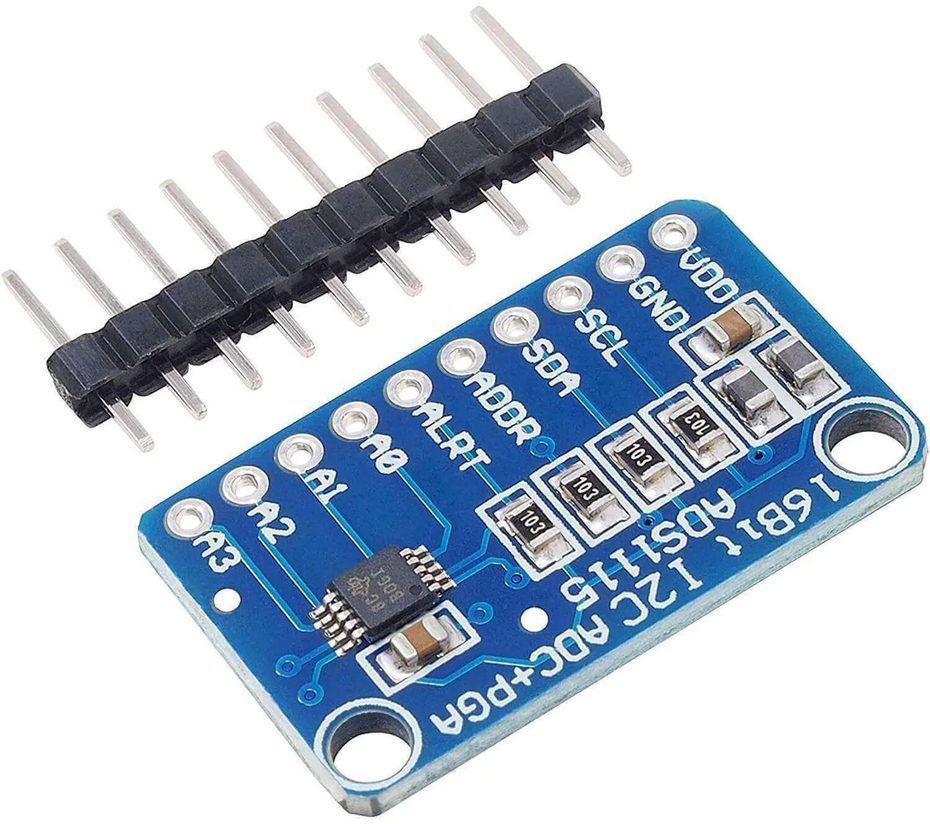
\includegraphics[width=0.35\textwidth]{images/sensors/ads1115.png}\hfill
    \caption{Modulo ADS1115.}
\end{figure}

\textbf{SENSTREE G1/2 CF-B7}\footnote{Link al venditore: \href{https://www.amazon.it/Interruttore-Misuratore-Contatore-Flussometro-Temperatura/dp/B07QNMZ7ZK}{https://www.amazon.it/AZDelivery-CFB7}}: il sensore del flusso d'acqua è costituito da un corpo in rame, un rotore dell'acqua, un magnete e un sensore ad effetto hall. Quando l'acqua scorre attraverso il rotore, questo inizia a girare insieme al magnete. La rotazione del campo magnetico attiva il sensore Hall, il quale emette onde quadre cioè impulsi. Ad ogni giro si avrà un certo volume di acqua che scorre, così come un determinato numero di onde quadre emesse. Pertanto, possiamo calcolare il flusso d'acqua contando il numero di onde quadre.

La formula per il calcolo del flusso d'acqua equivale a:
\[l_{hour} = \frac{flow_{frequency} \cdot 60}{11}\]

Sapendo che, nel caso di CF-B7, il sensore Hall genera 660 impulsi per ogni litro d'acqua, quindi ogni impulso corrisponde a $\frac{1}{660}$ litri. Detto ciò è possibile ricavare il volume totale ($V_{total}(L)$) di liquido che fluisce attraverso il sensore ad un certo tempo $t$, sfruttando il numero di impulsi:
\[V_{total}(L) = N \cdot \frac{1}{660}(L) \]

Inoltre, il volume precedente può essere calcolato anche come $water flow rate(Q - unit L/s)$ moltiplicato per il tempo $t$:
\[V_total(L) = Q(L/s) \cdot t(s) \]

Quindi, si ottiene:
\begin{gather*}
    N \cdot 1/660 = Q(L/s) \cdot t(s) \\
    N/t = 660 \cdot Q(L/s)
\end{gather*}

Infine, siccome $\frac{N}{t}$ equivale alla frequenza $f$:
\begin{gather*}
    f = 660 \cdot Q(L/s) \\
    Q(L/s) = \frac{f}{660} \\
    Q(L/min) = \frac{f \cdot 60}{660} = \frac{f}{11} \\
    Q(L/hour) = \frac{f \cdot 60 \cdot 60}{660} = \frac{f \cdot 60}{11} 
\end{gather*}

\begin{table}[H]
    \centering
    \begin{tabular}{|l|l|}
    \hline
    \textbf{Caratteristica} & \textbf{Descrizione}                \\ \hline
    Alimentazione           & 5$\sim$15 V                         \\ \hline
    Pressione massima acqua & 1,75 MPa                            \\ \hline
    Portata                 & 1$\sim$25L/min                      \\ \hline
    Sensore di temperatura  & NTC 3950 R25 = 50 K.                \\ \hline
    Intervallo di errore    & (1$\sim$30L\textbackslash MIN) ±3\% \\ \hline
    Frequenza               & F=(11*Q) Q=L/MIN ±3\%                 \\ \hline
    Temperatura dell'acqua  & $\leq$ 120°C                              \\ \hline
    Dimensioni              & 65 x 30 x 28 mm                     \\ \hline
    \end{tabular}
\end{table}

\begin{figure}[H]
    \centering
    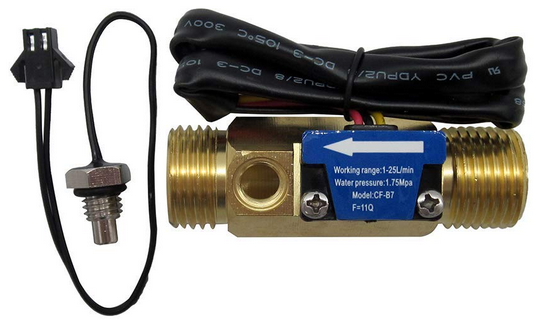
\includegraphics[width=0.35\textwidth]{images/sensors/cfb7.png}\hfill
    \caption{Modulo CF-B7.}
\end{figure}

\subsubsection{Software}
Come già anticipato le funzionalità della control unit sono state raccolte nei sottodomini Guest Authorization e Room Monitoring. Il primo definisce la gestione del \textit{token} di autorizzazione mentre la seconda descrive la logica di calcolo ed invio dei consumi.
% Dato un discreto numero di concetti di dominio da modellare, ci si è avvalsi del \textit{domain model pattern}. Infatti la business logic viene espressa in termini di:

%     value objects: utilizzati per rappresentare il token di autorizzazione e le varie tipologie di misurazioni (temperatura, corrente, ecc.);
%     entities: sfruttate per definire il concetto di rilevazione (detection) e sensore;
%     domain services: impiegati per modellare la logica di persistenza del token corrente (TokenRepository).

% Il pattern adottato prevederebbe altri elementi costitutivi, come gli aggregators, ma il loro impiego non è stato necessario dato il livello di complessità del dominio.
Inoltre la struttura dell'applicativo è sostenuta da una architettura esagonale (Figura \ref*{clarc}), la quale garantisce caratteristiche quali:
\begin{itemize}
    \item \textit{modularità}: le regole operative possono essere collaudate indipendentemente dalla UI, dal database o qualsiasi altro elemento esterno;
    \item \textit{indipendenza dai framework}: la scelta dei framework ricade solamente sull'ultimo strato dell'architettura, così da utilizzare questi come semplici strumenti evitando di sottostare a specifici vincoli;
    \item \textit{indipendenza dal database}: la business logic non è legata nè a un singolo database nè ad una specifica tipologia.
\end{itemize}

Tutto questo è reso possibile dal rispetto della "regola della dipendenza", la quale sostiene che le dipendenze presenti nel codice sorgente devono puntare solo all'interno, verso le politiche di alto livello. Nella pratica, alcune classi degli strati più esterni vanno ad implementare interfacce definite in quelli più interni. Infatti, la comunicazione con i servizi esterni avviene per mezzo di \textit{adapter} (interfacce) descritti internamente ed opportunamente concretizzati nell'ultimo livello. Inoltre questa tipologia di architettura consente di delineare un confine netto tra i due sottodomini, separando questi in due moduli distinti.
%
\begin{figure}[H]
    \centering
    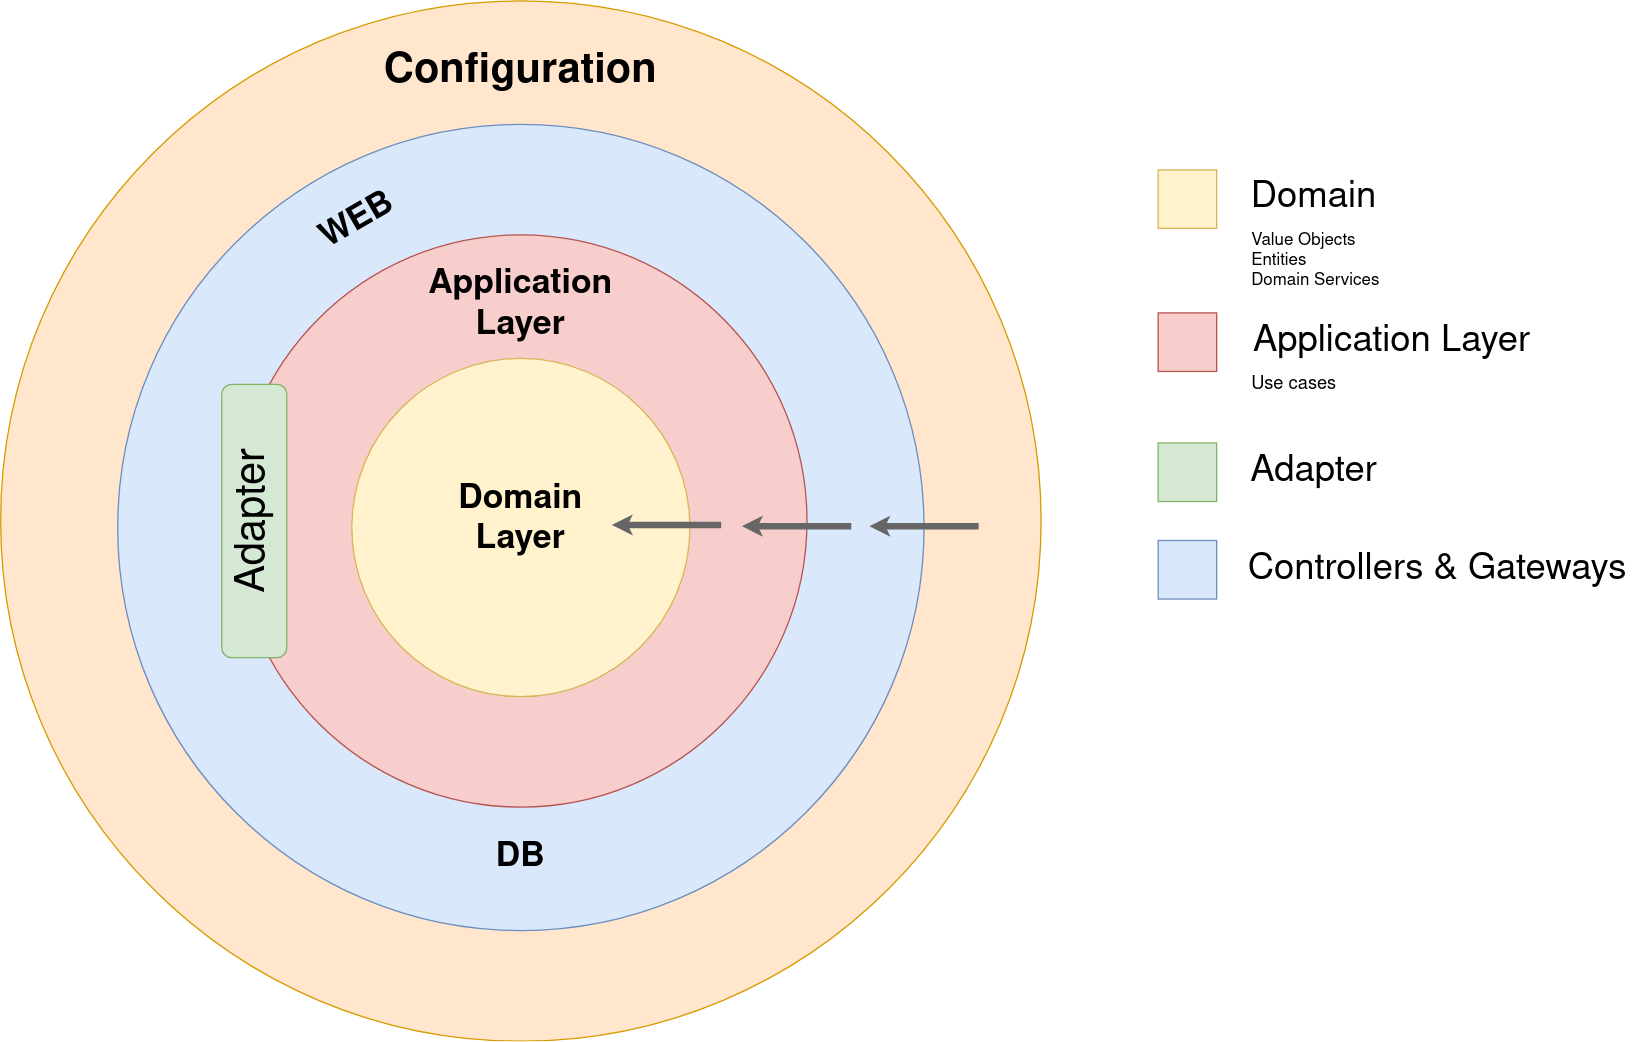
\includegraphics[width=\textwidth]{images/cl-architecture.png}\hfill
    \caption{\label{clarc}Rappresentazione grafica dell'architettura esagonale.}
\end{figure}
%Si può quindi dire che la progettazione della control unit è il risultato della combinazione della terminologia definita dall'ubiquitous language, con gli elementi del domain model pattern ed i concetti dell'architettura esagonale (Figura \ref{cu-uml}).%
Di particolare interesse è la definizione dello strato \textit{core} mediante casi d'uso, questi permettono di orchestrare i flussi di dati da e verso le entità, rimanendo aderenti agli schemi elaborati durante la fase di analisi. In Figura \ref{cu-uml} vengono schematizzati tutti i concetti principali di dominio, alcuni di questi sono semplici contenitori statici di valori (es. \texttt{Resistance}, \texttt{Current}, \texttt{Token}, ecc.) mentre altri definisco la logica dei casi d'uso e necessitano di un rapido approfondimento:
\begin{itemize}
    \item \texttt{EnvironmentUseCases}: racchiude la logica relativa al rilevamento dei fattori ambientali tramite i sensori di flusso dell'acqua, luminosità, temperatura e umidità;
    \item \texttt{ConsumptionUseCases}: come si evince dal nome, si occupa della raccolta dei consumi idrici ed elettrici;
    \item \texttt{AuthorizationUseCases}: set di funzionalità fondamentali per l'avvio della centralia, la ricezione/comunicazione del \textit{token} d'accesso e l'implementazione del protocollo di comunicazione tra la \textit{control unit} e uno smartphone nelle vicinanze.
\end{itemize}
\begin{figure}[H]
    \centering
    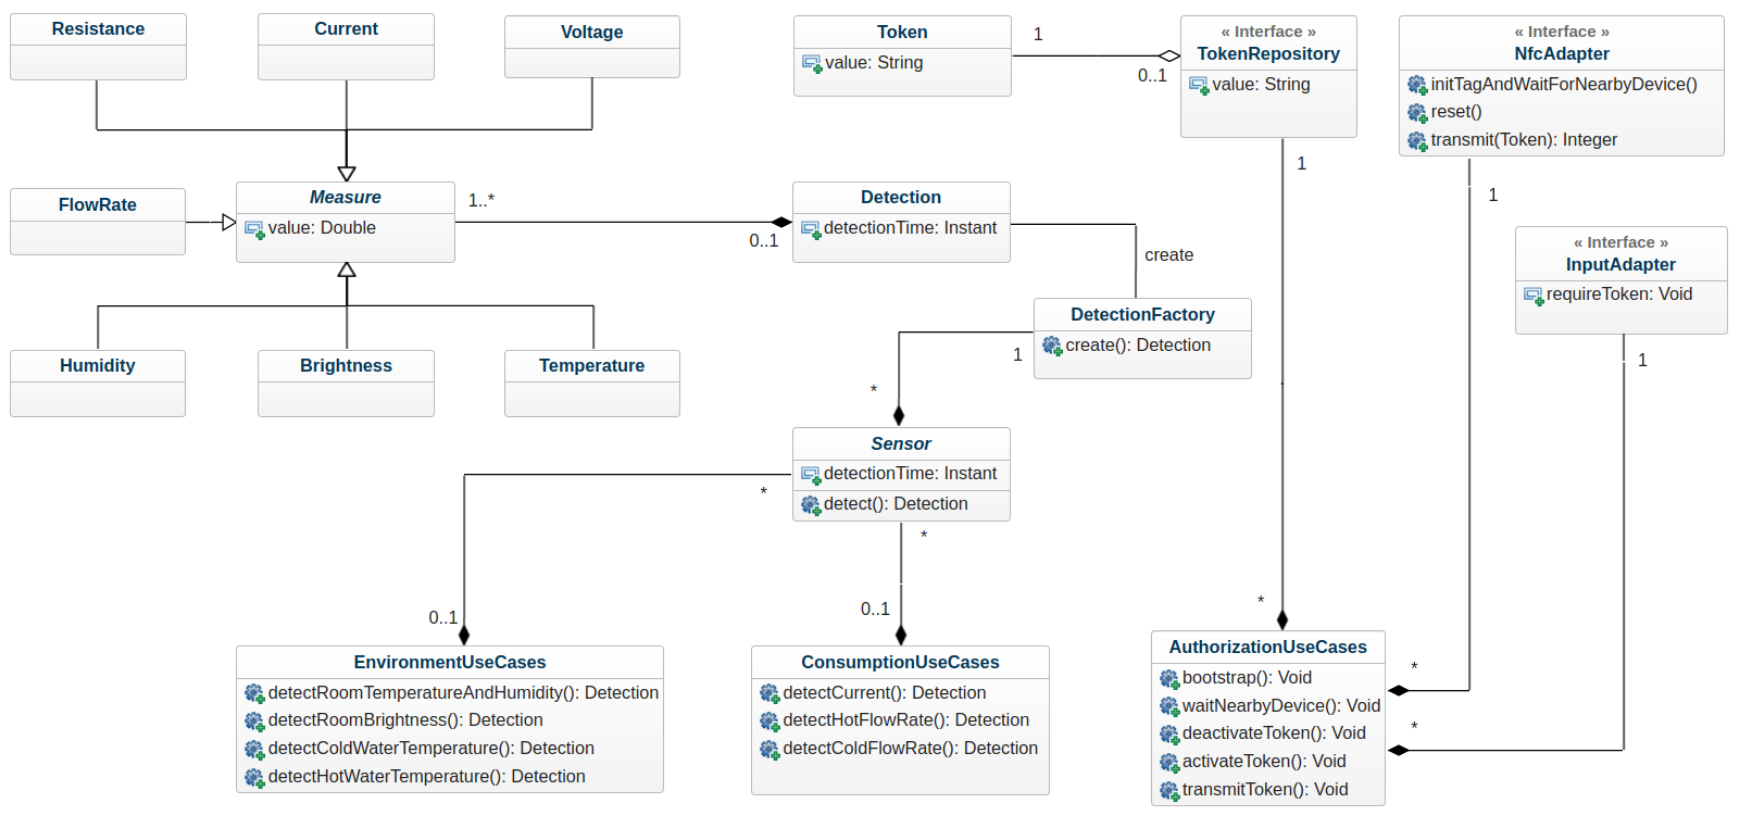
\includegraphics[width=\textwidth]{images/cu-uml.png}\hfill
    \caption{\label{cu-uml}Modellazione dei concetti di dominio tramite UML delle classi.}
\end{figure}
Nel caso delle rilevazioni, i dati prodotti vengono assegnati ad una specifica istanza di \texttt{Detection} che, oltre includere il valore rilevato, è associata alla data di creazione e ad un \textit{id} che la identifica univocamente. 
%
\begin{figure}[H]
    \centering
    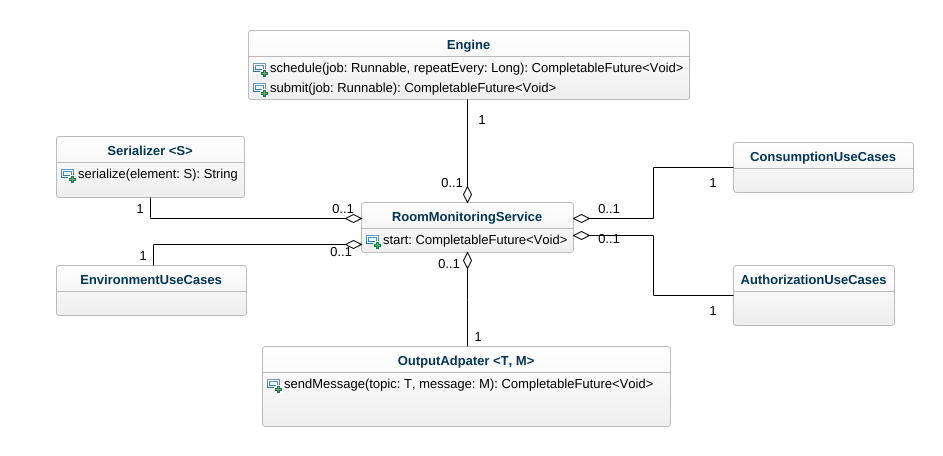
\includegraphics[width=\textwidth]{images/room-monitoring-serivce.png}\hfill
    \caption{\label{rm-uml}Diagramma UML delle classi (\texttt{RoomMonitoringService}).}
\end{figure}
%
Infine la logica di monitoraggio della stanza (\textit{Room Monitoring}) è racchiusa all'interno della classe \texttt{RoomMonitoringService} (Figura \ref*{rm-uml}). Questa, tramite un proprio flusso di controllo, esegue periodicamente (ogni 5 secondi) ed in maniera concorrente tutti i rilevamenti necessari (consumi e ambiente), interrompendoli nel caso di superamento del \textit{timeout}. Una volta ottenuti tutti i risultati, questi vengono prima serializzati grazie un'istanza di \texttt{Serializer} e successivamente comunicati verso l'esterno tramite l'\texttt{OutputAdapter}. Data la natura concorrente del servizio, si è scelto di schematizzarne il comportamento attraverso un diagramma di stato (Figura \ref*{rm-uml-state}).

\begin{figure}[H]
    \centering
    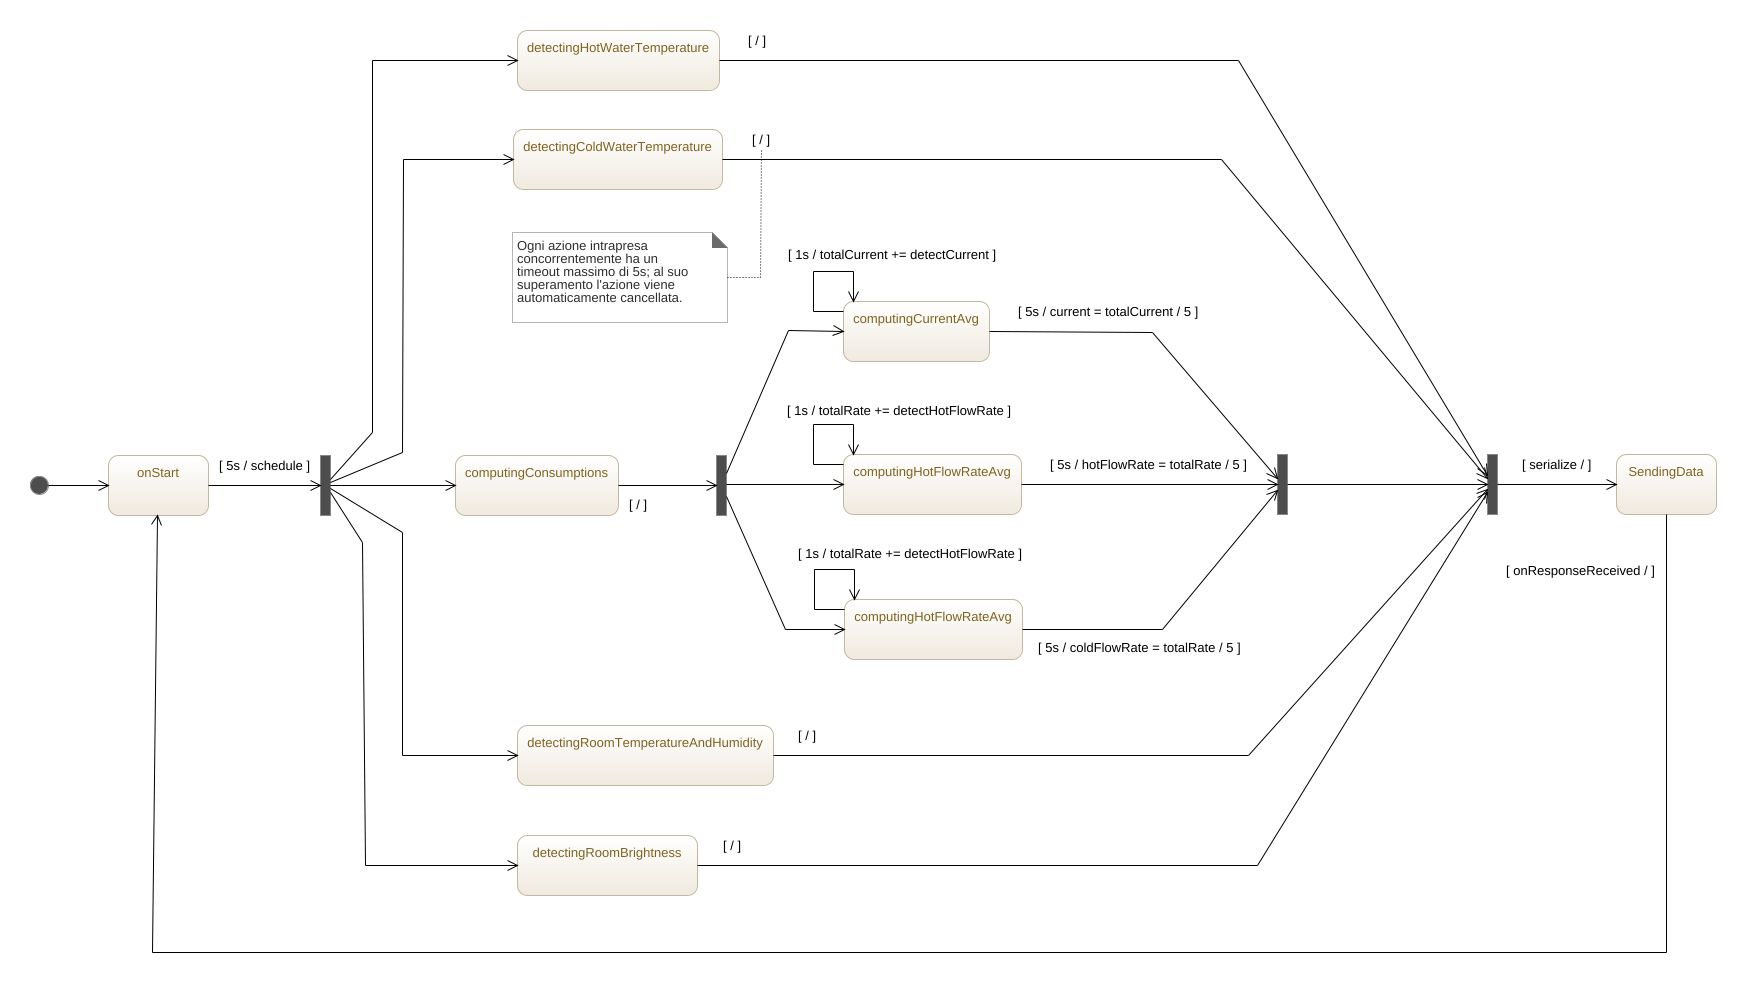
\includegraphics[width=\textwidth]{images/room-monitoring-service-state-diagram.jpeg}\hfill
    \caption{\label{rm-uml-state}Diagramma UML di stato (\texttt{RoomMonitoringService}).}
\end{figure}

\newpage